\documentclass[tikz]{standalone}
\usepackage{pgfplots}
\pgfplotsset{compat=1.15}
\usepackage{mathrsfs}
\usetikzlibrary{arrows,calc}
\usepackage{tkz-euclide}

\pagestyle{empty}

\definecolor{AngleClr}{rgb}{0,0.39215686274509803,0}
\definecolor{ShapeClr}{rgb}{0.6,0.2,0}

\begin{document}

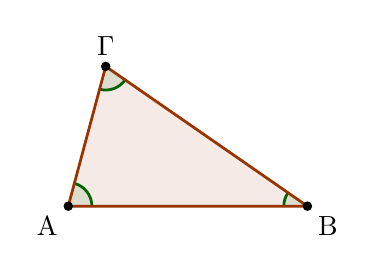
\begin{tikzpicture}[scale=.75]
\tkzSetUpLine[line width=1pt,color=black]
\tkzSetUpPoint[fill=black]

\tkzDefPoints{0/0/A,4.05/0/B}
\tkzDefPoint(75:2.45){C}

\tkzFillPolygon[fill=ShapeClr,fill opacity=0.1](A,B,C)

\tkzFillAngles[fill=AngleClr,size=.4,fill opacity=0.1](C,B,A B,A,C A,C,B)
\tkzMarkAngles[line width=1pt,size=.4,color=AngleClr](C,B,A B,A,C A,C,B)

\tkzDrawPolygon[color=ShapeClr](A,B,C)

\tkzDrawPoints[size=3](A,B,C)
\tkzLabelPoint[below left](A){$\rm A$}
\tkzLabelPoint[below right](B){$\rm B$}
\tkzLabelPoint[above](C){$\rm \Gamma$}

\end{tikzpicture}
\end{document}
